\chapter{Les contrats vus à travers l'énergie}
\section{Le Fonctionnement des marchés de gros de l'électricité}
\subsection{L’organisation de l’opérateur historique avant la libéralisation}
\begin{figure}[hbt!]
    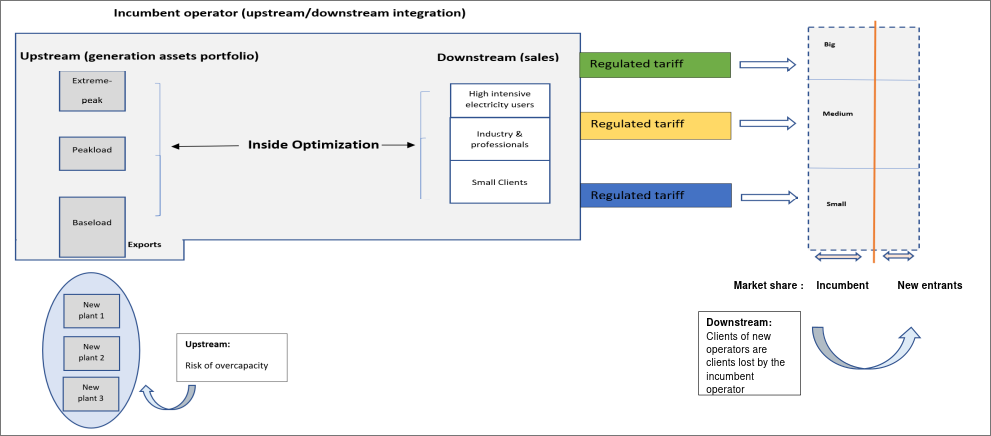
\includegraphics[scale=0.4]{Pics/marche_de_l_electricite_avant_liberalisation.png}
\end{figure}
\newpage
\subsection{Les business models}
\subsubsection{Stand alone model}
Modèle ou les fournisseurs d'électricité sont indépendants du réseau principal. Ce business model est conçu pour fonctionner dans des endroits isolés. Exemple d'UEM pour le réseau de Metz. \newline
C'est le modèle qu'a adoptée la commisison en 2007 pour les marchés de gros.
\begin{figure}[hbt!]
    \centering
    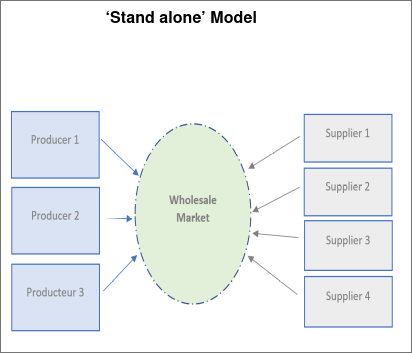
\includegraphics[scale=0.7]{Pics/Stand_alone_model.png}
\end{figure}
\newpage
\subsubsection{Fully Integrated Utilities}
Services publics entièrement intégrés. L'opérateur assure toute la chaine d'approvisionnement de l'électricité de manière centralisée, de la production jusqu'à la distribution aux clients finaux. S'oopose aux modèles fragmentés ou les différents segments sont réalisés par différentes entités.
\begin{figure}[hbt!]
    \centering
    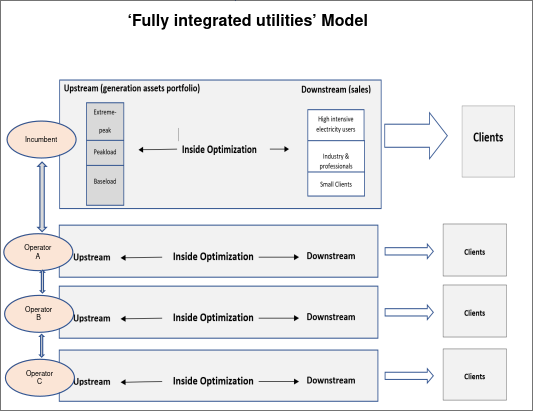
\includegraphics[scale=0.7]{Pics/Fully_integrated_model.png}
\end{figure}
\newpage
\section{La crise des prix pour le marché de gros de l'électricité}
Ordre de mérite :
\begin{figure}[hbt!]
    \centering
    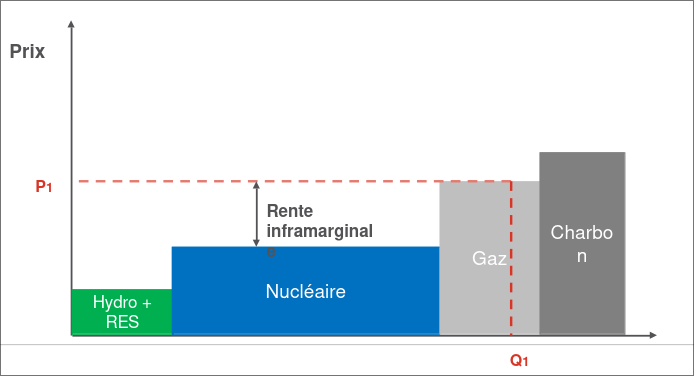
\includegraphics[scale=0.5]{Pics/ordre_de_merite.png}
\end{figure}
\begin{figure}[hbt!]
    \centering
    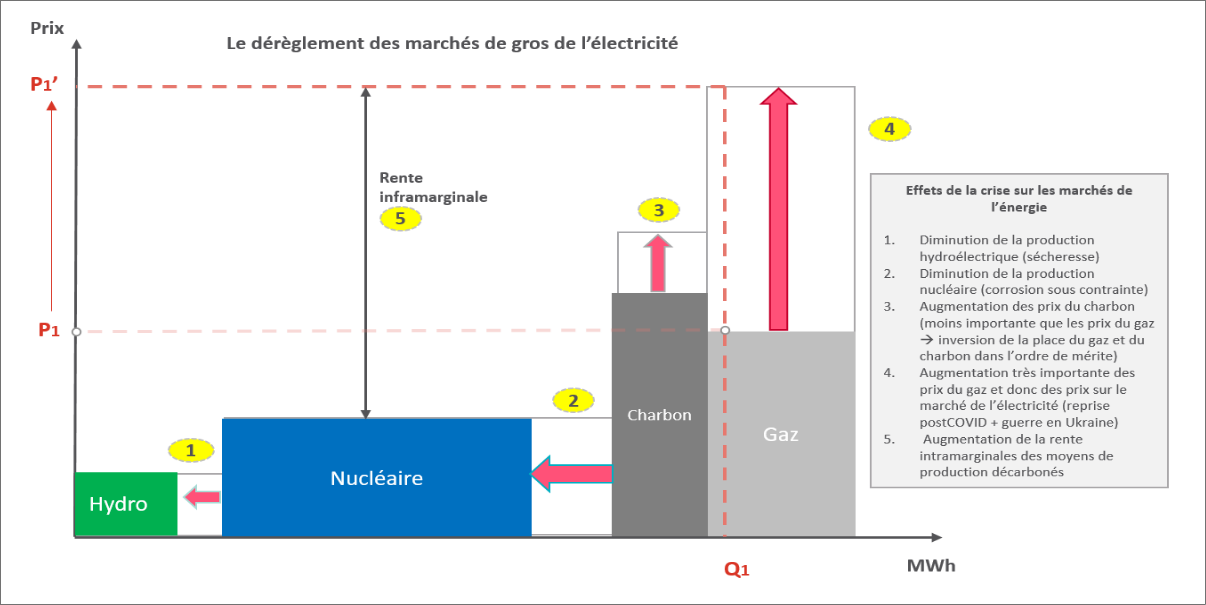
\includegraphics[scale=0.35]{Pics/dereglement_prix_elec.png}
\end{figure}
\newpage
\begin{figure}[hbt!]
    \centering
    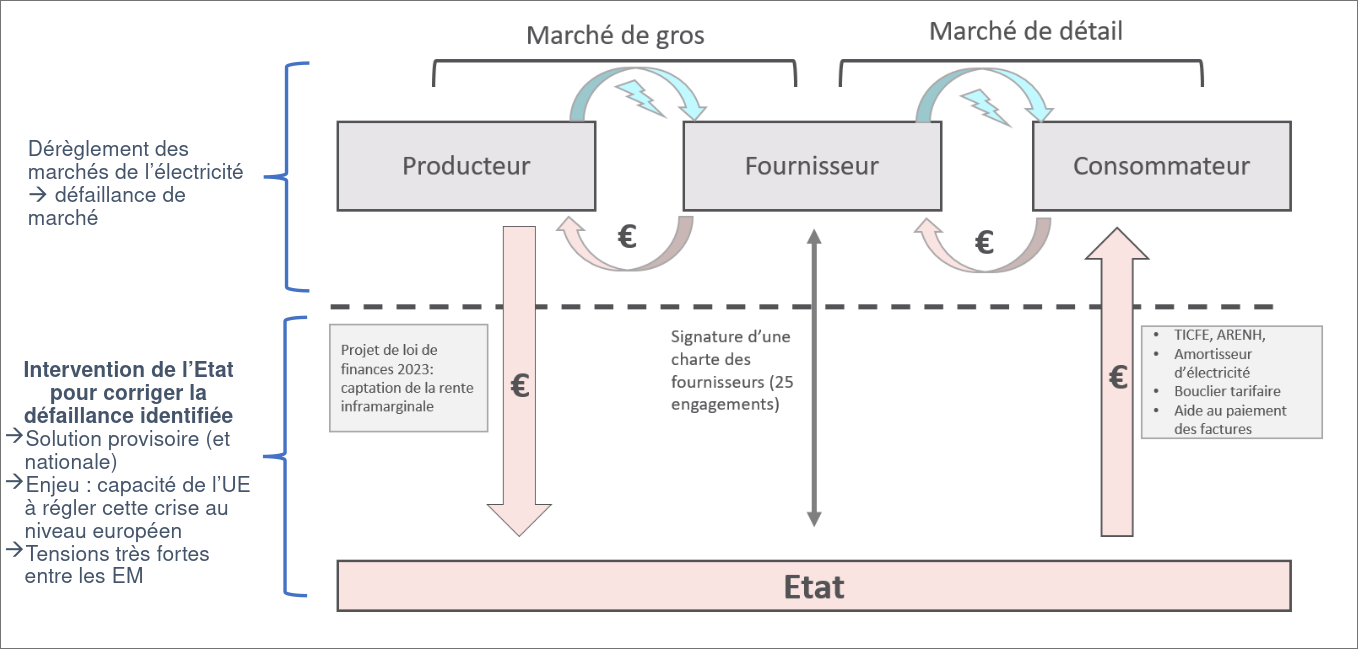
\includegraphics[scale=0.3]{Pics/fiscalite_et_surprofits.png}
\end{figure}
Solutions mises en place pour la protection des consommateurs sur la hausse des prix :
\begin{itemize}
    \item Règlement du conseil de l'UE \footnote{Article 6: 1. « Les recettes issues du marché obtenues par les producteurs d’électricité à partir des sources visées à l’article 7, paragraphe 1, sont plafonnées à un maximum de 180 EUR par MWh d’électricité produite ».}
    \item Loi n°2022-1726 du 30 décembre 2022 : \textbf{loi de finance pour 2023} en France $\implies$ \textbf{Article 54} \newline
\end{itemize}
Fonctionnement de l'article 54 : 
\begin{figure}[hbt!]
    \centering
    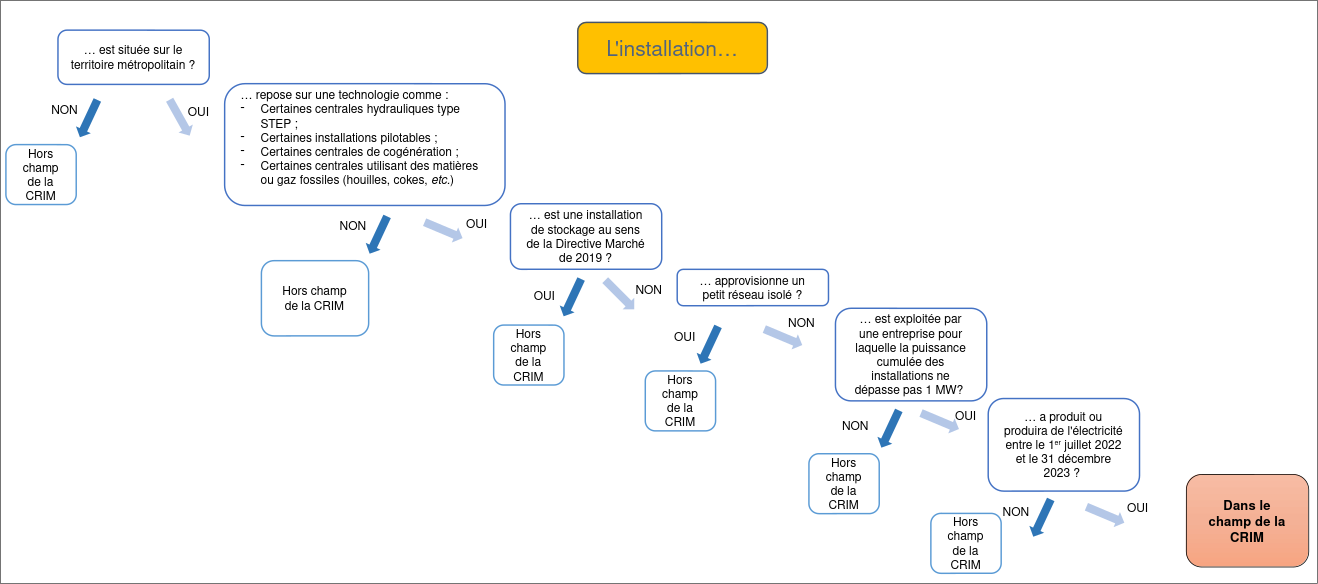
\includegraphics[scale=0.3]{Pics/principe_art_54.png}
\end{figure}
\newpage
« Le montant de la contribution est égal à la fraction des revenus de marché de l'exploitant de l'installation excédant un seuil forfaitaire. Cette fraction fait l'objet d'un abattement de 10 \% »
\begin{center}
    \Large{\fbox{$
    MF = Rm - F - D
    $}}
\end{center}
\begin{itemize}
    \item $MF$ : marge forfaitaire
    \item $Rm$ : revenu de marché
    \item $F$ : forfait
    \item $D$ : déductions finales
\end{itemize}
\section{Fiscalité en market design}
Proposition de la commisison E de réformer le Fonctionnement de marché de gros (2023) : \newline
Il y a des problèmes :
\begin{itemize}
    \item Centralisation excessive du larché de gros à court terme
    \item Potection des consommateurs de la volatilité des prix à court terme
    \item Discussions sur les contrats long terme : ils étaient jusqu'alors perçus comme des freins à la libéralisation du secteur de l'électricité
\end{itemize}
\newpage
\section{Les contrats long terme}
\subsection{Les CFD (contract for difference)}   
C'est un contract entre un investisseur et un courtier : l'investisseur spécule sur la hausse ou la baisse d'un bien. Si la valeur du bien augmente, le courtier paye la différence de prix entre le début et la fin du contrat. Si la valeur du bien diminue, c'est l'investisseur qui compense.
\begin{figure}[hbt!]
    \centering
    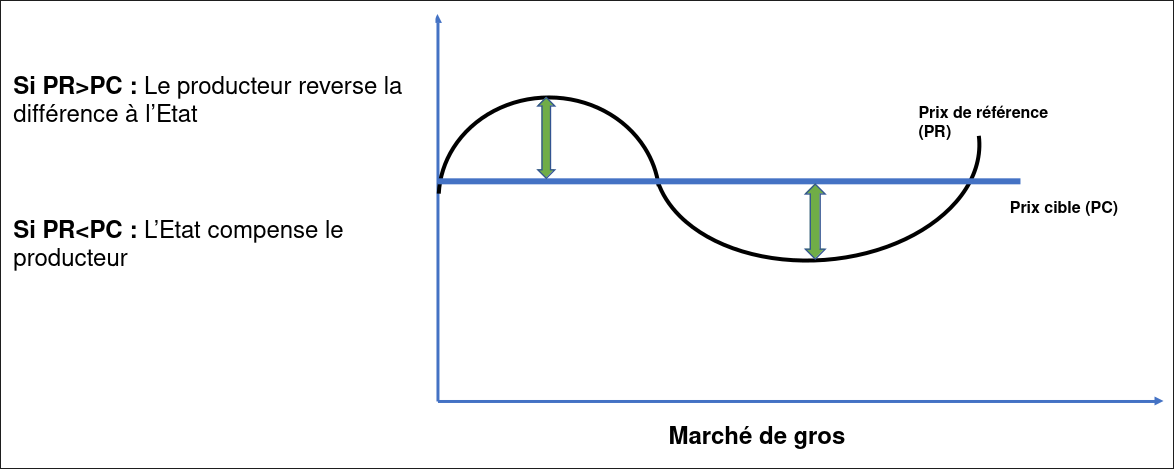
\includegraphics[scale=0.3531]{Pics/CFD_fonctionnement.png}
\end{figure}
\subsection{Les PPA (Power Purchase Agreement)}
C'est un contrat entre un client et un fournisseur d'électricité. Le fournisseur s'engage à produire une certaine quantité d'énergie pendant que le client s'engage à payer une certaine somme, correspondant à cette quantité d'énergie indexée sur le prix de l'électricité ou bien un prix fixe. Si le marché fluctue, ils compensent la différence.
\newpage
\begin{figure}[hbt!]
    \centering
    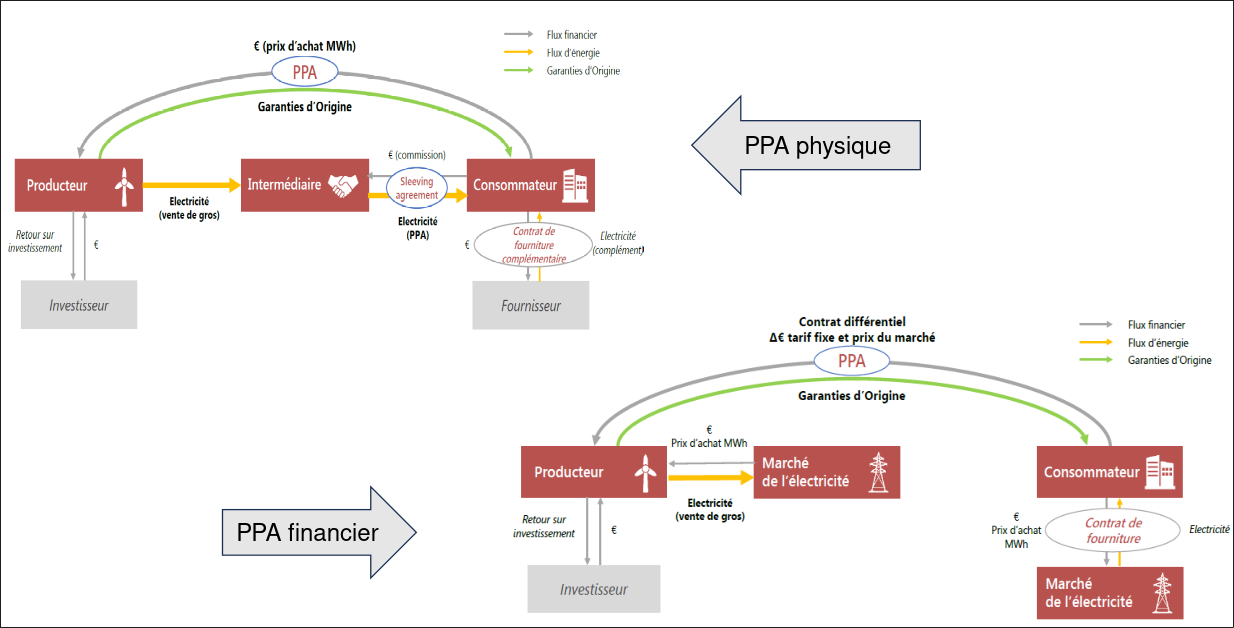
\includegraphics[scale=0.3531]{Pics/PPA_physique_et_PPA_financier.png}
\end{figure}
\subsection{Risk sharing contract}
Contrat de partage de risques. Les écarts entre la consommation cible sont compensés par les deux parties (consommateur et fournisseur). Ces parties peuvent êtres inégales. Par exemple : quand la consommation est trop grande par rapport à la cible, le client paye $2/3$ de l'écart et $1/3$ pour le fournisseur. A l'inverse, si la cible est surévaluée et le consommateur consomme finalement moins que la cible, le fournisseur rembourse $4/5$ de la différence.
\subsection{Purely supply contract}
Contrat de fourniture pure. L'approvisionnement de l'énergie est purement définie, c'est-à-dire qu'une quantité d'énergie est délivrée et payée, sans considérer la part de risques, car il n'y a pas de cible prévisionnelle : uniquement une quantité payée et effectivement consommée.
\newpage
\section{Liquidité des marchés de gros}
\textbf{Liquidité : facilité de vendre et d'acheter une grosse quantité d'électricité sans affecter les prix du marché.} Le manque de liquidité cause une volatilité conséquente \footnote{Taux de variation des prix en fonction du temps} \newline
Les PPA ne sont pas la bonne solution pour la liquidité, c'est pour cela que la Commisison Européenne favorise le stand-alone model. Cependant, le modèle du stand-alone force le marché de gros, qui lui-même est un marché très volatile \footnote{problèmes de stockage liés à l'énergie électrique}. De plus, le stand-alone model n'es pas optimal d'un point de vue industriel et colectif \footnote{Rapport Champsaur}. Il faut alors que la Commisison se penche sur d'autres modèles que le stand alone : il ne doit pas être le seul modèle.
\section{La nécéssité d'évolution dans l'appréciation des contrats long terme pour la Comission}
\begin{figure}[hhbt!]
    \centering
    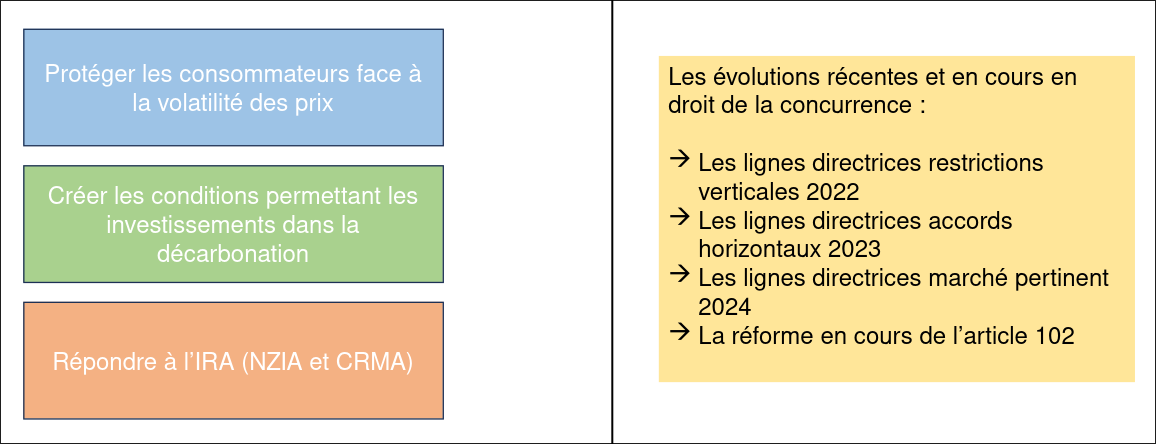
\includegraphics[scale=0.35]{Pics/evolution_contrat_long_terme.png}
\end{figure}